\documentclass[../notesdecours.tex]{subfiles}
\usepackage{enumitem}
\usepackage{cancel}
\usepackage{calrsfs}

\begin{document}

\chapter{Applications des postulats de la Mécanique Quantique}

\section{Interféromètre de Mech-Zehnder}
L'interféromètre de Mach-Zehnder est un exemple d'expérience qui est tiré de l'optique ; nous allons nous aider du formalisme de la mécanique quantique pour mettre en évidence l'aspect ondulatoire ou corpusculaire du photon dans cette expérience. \\
L'idée que nous allons souligner est la suivante : tant que le photon reste sous sa forme ondulatoire dans le dispositif, il interfère avec lui-même, et il se peut qu'un seul des deux détecteurs ne s'activent. A partir du moment où le photon prend sa forme corpusculaire dans le dispositif (parce qu'il est mesuré, perturbé), l'interférence n'a pas lieu et les deux voies de sortie peuvent être activées. 

\textcolor{red}{Schéma à modifier}
\begin{center}
    \begin{figure}[h]
    \centering
    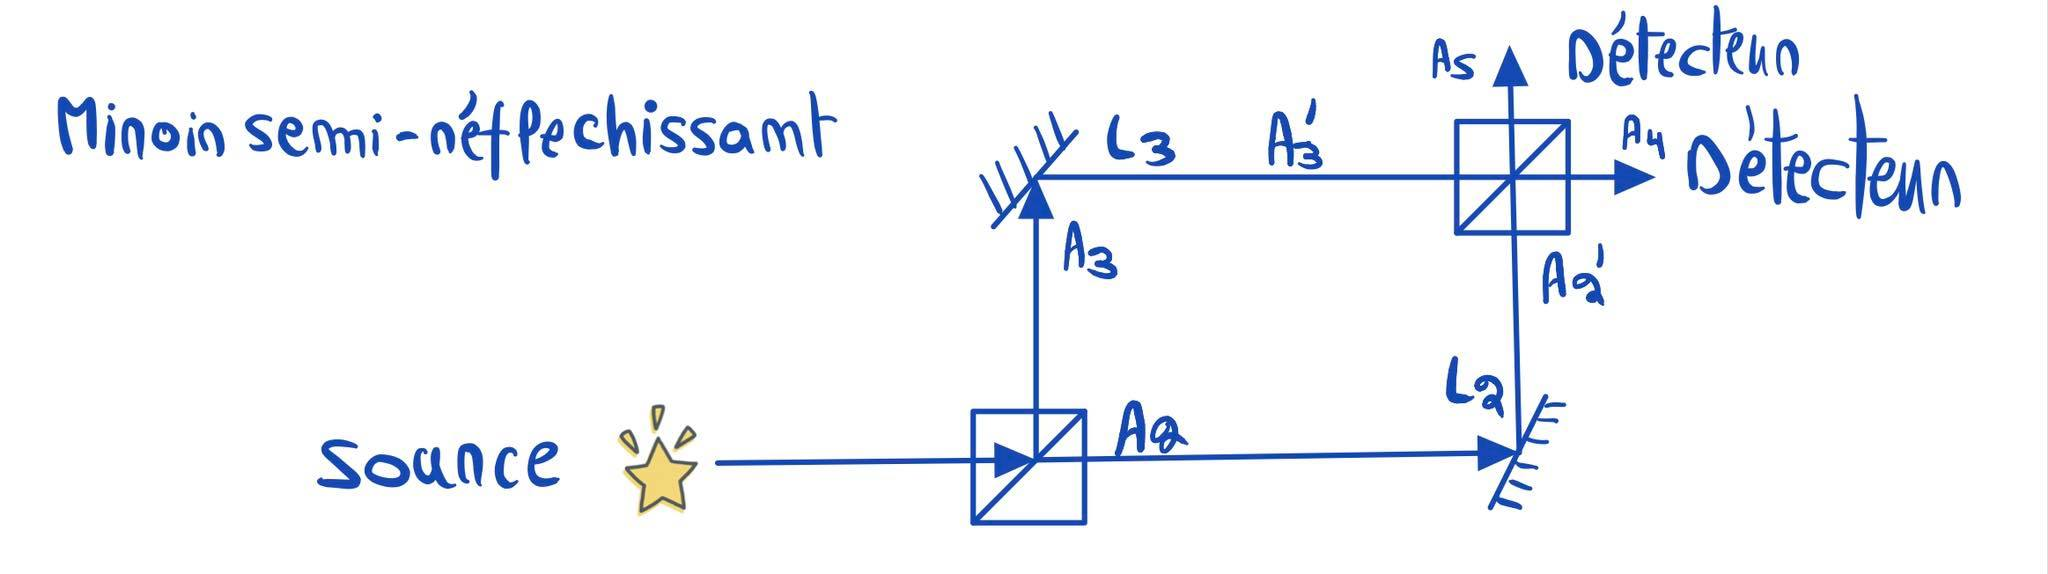
\includegraphics[width=0.80\textwidth]{Mach-Zehnder.png}
    \caption{Schéma du dispositif. $L_2$ et $L_3$ sont les longueurs totales du chemin 1, respectivement 2 suivi par la lumière. }
    \label{Mach-Zehnder}
    \end{figure}
\end{center}

\subsection{Etude classique (la lumière classique est de nature ondulatoire)}

Le faisceau lumineux, initialement divisé en deux par un premier beam-splitter (noté BM par la suite, c'est un miroir semi-réfléchissant), se recombine par les miroirs : en arrivant au deuxième BM, ils interfèrent constructivement lorsqu'ils sont en phase. \\

La différence de phase peut se manifester lorsque : 
\begin{itemize}[label = \textbullet]
    \item il y a une différence de distance parcourue par chaque faisceau ; 
    \item il y a un changement d'indice de réfraction le long du trajet (mais ce n'est pas le cas ici)
\end{itemize}

Ces phénomènes d'interférences interviennent également en fibres optiques : 
\textcolor{red}{Schéma} 
\newline Il y a interférence en fonction de la longueur relative des chemins. \\

Effectuons à présent une étude quantitative du problème pour déterminer l'intensité des faisceaux mesurée aux détecteurs lorsque le système est considéré d'un point de vue classique. \\

Considérons tout d'abord un seul BM.

\begin{center}
    \begin{figure}[h]
    \centering
    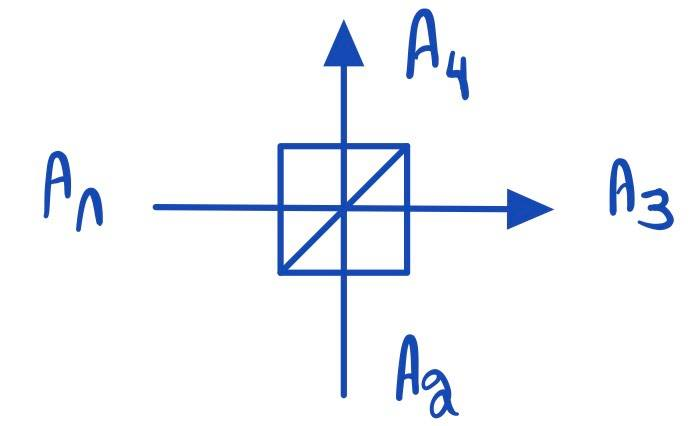
\includegraphics[width=0.50\textwidth]{bean.png}
    \caption{Schéma d'un beam-splitter ; les ondes incidentes arrivent de $A_1$ et $A_2$}
    \label{Interferometre}
    \end{figure}
\end{center}

On considère également deux ondes incidentes qui sont des ondes planes de même fréquence mais d'amplitude différente $A_1$ et $A_2$ : 
\begin{align}
    A_1(t) &= A_1 e^{-i\omega t} \notag \\
    A_2(t) &= A_2 e^{-i\omega t}
\end{align}\label{A1 et A2}

Ecrivons ensuite les ondes résultantes $A_3(t)$ et $A_4(t)$ comme : 
\begin{align}
    A_3(t) &= c \; A_1(t) + i s \;A_2(t) \notag \\
    A_4(t) &= is \; A_1(t) + c \; A_2(t) 
\end{align}\label{A3 et A4}
où nous pouvons prendre $c = \cos(\theta)$ et $s = \sin(\theta)$. 

En effet, cela a du sens d'écrire $A_3(t)$ et $A_4(t)$ de cette manière-ci car : \begin{itemize}[label = \textbullet]
    \item les équations de l'électromagnétisme sont linéaires (une combinaison linéaire d'ondes planes de même fréquence reste bien une onde plane) ; 
    \item Si on suppose que l'on envoie deux faisceaux de lumières sur un miroir semi-transparent d'intensité $I_1 = \left| A_1 \right|^2$ et $I_2 = \left| A_2 \right|^2$, et supponsons qu'il n'y a pas de perte : alors $I_1 + I_2 = I_3 + I_4$. Les amplitudes sortantes et entrantes sont reliées par une matrice, et c'est la conservation des intensités qui impliquent que cette matrice est unitaire. Ainsi, dans les relations \eqref{A3 et A4}, on peut choisir un des coefficients, par exemple $\left| c \right|^2$ en choisissant un miroir semi-transparent. Le coefficient $\left| s \right|^2$ est alors fixé par la relation $\left| c \right|^2 + \left| s \right|^2 = 1$. 
    \newline Il reste également une liberté de phase : en effet, il est possible de redéfinir la phase de $A_1 = e^{i\Phi} A_1'$ ; il en est de même pour les autres faisceaux. 
\end{itemize}

Notons que si l'on a une onde qui parcourt une distance L d'un point A à un point A', alors une phase de $kL$ s'introduit dans l'expression de l'onde en ce point A' : 
\begin{align}
    \mbox{en A : } A(t)&= Ae^{-i\omega t} \\
    \mbox{en A': } A'(t)&= A e^{-i\omega t} e^{ikL}
\end{align}\label{dephasage} \\

\textit{Remarques :} 
\begin{enumerate}
    \item Par convention, nous supposerons que l'onde transmise ne subit aucun déphasage, tandis que l'onde réfléchie subit un déphasage de $\pi /2$ (d'autres conventions sont possibles) ; 
    \item Lorsqu'un faisceau de lumière arrive à un détecteur, ce que ce dernier mesure est un courant électrique $I(t) = e \left| A(t) \right|^2$. 
\end{enumerate}

Considérons à présent l'interféromètre qui contient 2 BM. \textcolor{red}{schéma pour représenter les $A_i$ à chaque entrée/sortie d'un BM}. 

Dans ce cas-ci, il n'y a qu'une seule source de lumière et le faisceau incident est donné par : $A(t) = Ae^{-i\omega t}$ (l'intensité du faisceau à la source est alors $I_0 = \left| A(t) \right|^2 = \left| A \right|^2$). 
Par les relations \eqref{A3 et A4}, et en choisissant $c = \frac{1}{\sqrt{2}}$ (qui n'est rien d'autre qu'un choix de phase pour simplifier les calculs) : \begin{align}
    A_2(t) &= \frac{A(t)}{\sqrt{2}} \notag \\
    A_3(t) &= i \frac{A(t)}{\sqrt{2}}
\end{align} 
Et par \eqref{dephasage}, on trouve au deuxième BM: 
\begin{align}
    A_2'(t) &= A_2(t) e^{ikL_2} \\
    A_3'(t) &= A_3(t) e^{ikl_3}
\end{align}
On note $\Delta \Phi = kL_3 - kL_2$ la différence de phase entre les deux ondes au deuxième BM. \\

En utilisant à nouveau les relations pour les ondes sortantes du BM, on trouve : 
\begin{align}
    A_4(t) &= \frac{A_3'(t)}{\sqrt{2}} + i \frac{A_2'(t)}{\sqrt{2}} = \frac{1}{\sqrt{2}} \left( A_3(t)e^{ikL_3} + i A_2(t) e^{ikL_2} \right) = i \frac{A(t)}{2} \left( e^{ikL_3} + e^{ikL_2} \right) \\
    A_5(t) &= i \frac{A_3'(t)}{\sqrt{2}} + \frac{A_2'(t)}{\sqrt{2}} = \frac{1}{\sqrt{2}} \left( iA_3(t) e^{ikL_3} + A_2(t)e^{ikL_2} \right) = \frac{A(t)}{2} \left( e^{ikL_2} - e^{ikL_3} \right) 
\end{align}

Ainsi, l'intensité des ondes aux détecteurs se trouve par : 
\begin{align}
    I_4 &= \frac{\left| A \right|^2}{4} \left| e^{ikL_3} + e^{ikL_2} \right|^2 \\ 
    I_5 &= \frac{\left| A \right|^2}{4} \left| e^{ikL_2} - e^{ikL_3} \right|^2
    \label{I4 et I5}
\end{align} \\

Développons le membre de droite de \eqref{I4 et I5} pour $I_4$ : 
\begin{align*}
    \left| e^ikL_3 + e^ikL_2 \right|^2 &= \left| e^{ikL_3} \right|^2 + \left| e^{ikL_2} \right|^2 + e^{ikL_3}(e^{ikL_2})^* + e^{ikL_2}(e^{ikL_3})^* \\
    &= 2 + 2\textit{Re}\left[ e^{ikL_3}(e^{ikL_2})^* \right] \\
    &= 2+2\left( \cos{kL_3} \cos{kL_2} + \sin{kL_2}\sin{kL_3} \right) \\
    &= 2 \left( \cos{(kL_3 - kL_2)} +1 \right) \\
    &= 4\cos^2{\frac{\Delta \Phi}{2}}
\end{align*}

Par un raisonnement similaire pour le membre de droite de $I_5$, nous avons finalement : 
\begin{align}
    I_4 &= \left| A \right|^2 \cos^2{\frac{\Delta \Phi}{2}} \\
    I_5 &= \left| A \right|^2 \sin^2{\frac{\Delta \Phi}{2}}
\end{align}
$$ \rightarrow I_4 + I_5 = \left| A \right|^2 = I_0 $$ 
Il y a bien conservation de l'intensité de l'onde émise, ce qui en fait était garanti par notre choix de phase car celui-ci faisait en sorte que $A_3(t)$ et $A_4(t)$ soient reliés à $A(t)$ par une transformation unitaire. 

\subsection{Etude quantique}

Avec le même dispositif, nous allons cette fois considérer une source d'\textbf{un seul photon}, plutôt qu'un faisceau de lumière. \\
Classiquement, il serait naturel de se dire que le photon étant indivisible, ne passe que par un des deux chemins. Il arriverait alors à un détecteur ou à l'autre, avec une probabilité qui dépend du coefficient de réflexion du miroir semi-réfléchissant. En réalité, il se peut qu'un seul des deux détecteurs s'activent ; il y aurait manifestement des interférences même lorsque le faisceau est réduit à un seul photon. Il devient donc nécessaire de faire appel à la mécanique quantique pour étudier cela. 

\paragraph{Description des \textbf{états quantiques} : }
Si le photon peut suivre plusieurs chemins, on dira que l'état est : 
\begin{equation}
    \ket{\psi} = \alpha\ket{1}+\beta\ket{2}+\gamma\ket{3}
\end{equation}\label{etat photon}
Avec $\left| \alpha \right|^2 + \left| \beta \right|^2 + \left| \gamma \right|^2 = 1$, et $\ket{i}$ pour $i \in \{ 1,2,3 \}$ est l'état du photon dans le chemin i. 

\paragraph{Beam-splitter :}
Un BM tel que décrit précédemment, induit une évolution donnée par : 
\begin{align}
    \ket{1} &\rightarrow c\ket{3} + is\ket{4} \notag\\
    \ket{2} &\rightarrow is\ket{3} + c\ket{4}
\end{align}\label{BM evolution}
Cette évolution est décrite par la matrice  $\begin{pmatrix}
c & is\\
is & c
\end{pmatrix}$ qui est unitaire unitaire (ce qui est cohérent par le postulat qui exprimer le fait que l'évolution des états se fait de manière unitaire).\\

\paragraph{Détecteur du photon :} \textcolor{red}{Schéma des détecteurs avec 2 chemins} Supposons que l'on mesure le photon dans la base $\ket{1}$ et $\ket{2}$. \\
Si l'état du photon est donné par $\ket{\psi} = \alpha\ket{1}+\beta\ket{2}$, alors les probabilités de détection seront données par : 
\begin{align}
    P(click 1) = \left| \alpha \right|^2 \notag \\
    P(click 2) = \left| \beta \right|^2 
\end{align}\label{proba_detection} 

\paragraph{Description quantique de l'interféromètre : }
La description de l'expérience découle en effet naturellement des points précédents durant lesquels on formalise l'expression des états du système, de l'évolution d'un état en passant par un BM, et des probabilités de détection d'un photon ;
\begin{description}
    \item Initialement : $\ket{\psi} = \ket{1} \equiv$ état d'un photon dans le chemin 1
    \item $\rightarrow$ 1er passage dans le BM : $\ket{\psi} = \frac{1}{\sqrt{2}} \ket{2} + \frac{i}{\sqrt{2}} \ket{3}$ 
    \item $\rightarrow$ Après avoir parcouru $L_2$ ou $L_3$ : $\ket{\psi} = \frac{e^{ikL_2}}{\sqrt{2}} \ket{2'} + i \frac{e^{ikL_3}}{\sqrt{2}} \ket{3'}$
    \item $\rightarrow$ 2ème passage dans le BM : par \eqref{BM evolution}, on a que : 
    \begin{align}
    \ket{3'} &\rightarrow c\ket{4} + is\ket{5} = \frac{1}{\sqrt{2}} \left( \ket{4} + \ket{5} \right) \notag\\
    \ket{2'} &\rightarrow is\ket{4} + c\ket{5} = \frac{1}{\sqrt{2}} \left( i \ket{4} + \ket{5} \right) 
    \end{align}
    Donc $\ket{\psi} = \frac{e^{ikL_2}}{\sqrt{2}} \ket{2'} + i \frac{e^{ikL_3}}{\sqrt{2}} \ket{3'}$ devient $\ket{\psi} = \frac{1}{2}\left( e^{ikL_2} - e^{ikL_3} \right) \ket{5} + \frac{i}{2} \left( e^{ikL_2} + e^{ikL_3} \right) \ket{4}$
    \item $\rightarrow$ Probabilité de détection : par \eqref{proba_detection}, on trouve : 
    \begin{align}
    P(click 4) &= \cos^2 \frac{\Delta \Phi}{2}\\
    P(click 5) &= \sin^2 \frac{\Delta \Phi}{2}
    \end{align}
\end{description}

\textbf{Le photon est simultanément dans les chemins 2 et 3.} On observe d'ailleurs que s'ils ne sont pas déphasés, \textit{i.e} $\Delta \Phi = 0$, alors P(click 4) = 1 : il y a une interférence constructive qui fait qu'avec probabilité 1, seul un détecteur va s'enclencher. Le photon agit donc bien comme une onde. \\

\paragraph{Modification d'un paramètre du dispositif :} Nous pouvons imaginer deux situations qui diffèrent de l'expérience initiale. \\

Premièrement, regardons ce qu'il se passe lorsqu'un des chemins est bloqué : \textcolor{red}{Schéma d'un chemin bloqué} \\
Dans ce cas-ci, il est clair que 
\begin{align*}
    P(D_2 click) &= 1/2 \\
    P(D_4 click) &= 1/4 \\
    P(D_5 click) &= 1/4
\end{align*}

Deuxièmement, on pourrait aussi supprimer le deuxième BM, et dans ce cas : \textcolor{red}{Schéma d'un BM en moins}
\begin{align*}
    P(D_4 click) &= 1/2 \\
    P(D_5 click) &= 1/2
\end{align*}

Dans ces deux derniers cas, les probabilités sont simplement données par le fait qu'il y ait autant de chance que le photon soit réfléchi qu'il soit transmis, en passant par un BM. Le photon ici agit donc comme une particule. 

\paragraph{\textit{Delayed choice experiment} (Wheeler-1978) :} Une question que l'on pourrait se poser est la suivante : "\textit{Est-ce que le photon sait-il d'avance ce qu'il doit faire ?}", autrement dit, selon les configurations du système, le photon décide-t-il d'agir comme une particule ou comme une onde ? \\
Par exemple, pourquoi pas enlever/remettre un BM, changer la phase $\Delta \Phi$, \textbf{après} que le photon soit entré dans l'interféromètre. Des expériences montrent cependant que le photon peut être simultanément onde et particule à la fois ; l'interprétation où l'on suppose que le photon "sait à l'avance ce qu'il doit faire" ne tient donc pas. 

\subsection{Elitzur-Vaidman \textit{"bomb tester"} (1993), expérience de pensée}

\textcolor{red}{petit schéma avec la bombe}\\
Soit $\mathcal{B} \equiv$ une bombe armée (explose si 1 seul photon touche le senseur), \\
et ${\mathcal{B^*}} \equiv$ une bombe non-armée (pas de senseur présent). \\

Supposons que l'on dispose de bombes armées et non-armées, mais indistinguables.\\
Comment pourrions-nous faire pour sélectionner une bombe armée ? \\

Disposons-nous d'un interféromètre, réglé tel que $\Delta \Phi = 0$. Par l'étude précédente de l'interféromètre, nous savons que $P(click 4) = 1$ et $P(click 5) = 0$. \\
Perturbons à présent le système en plaçant une bombe sur le chemin 2 ; autrement dit, cela revient à bloquer le chemin 2 si la bombe est armée, ou à ne rien faire si la bombe n'est pas armée ; 
\begin{itemize}
    \item Si la bombe n'est pas armée : $P(click 4) = 1$ ; $P(click 5) = 0$
    \item Si la bombe est armée : $P(Boum) = 1/2$ ; $P(click 4) = 1/4$ et $P(click 5) = 1/4$. 
\end{itemize}
Un click en 5 signalerait donc que l'on a une bombe armée de manière fiable, et elle n'a pas explosé! 

\section{Oscillations de neutrinos}
Une particule est dite élémentaire lorsque sa composition nous est inconnue. L'étude du comportement de ce type de particules fait l'objet de la physique des particules. Le plus récent modèle mathématique décrivant cette réalité est un résultat connu sous le nom de \textit{modèle standard des particules élémentaires}. Un exemple de telle particule est l'électron, rencontré dans les atomes. Il se trouve que le neutrino en est un autre exemple. Notons que la découverte de cette particule est extrêmement récente à l'échelle de l'histoire de la science et de l'humanité : elle a été prédite par Pauli en 1930, et ne fût observée pour la première fois qu'en 1956.\\

Une des propriétés fondamentales du neutrino est qu'elle n'intéragit que très faiblement avec la matière. Aussi, ceci explique pourquoi sa découverte n'est que très récente: il aurait auparavent été tout bonnement impossible de l'observer, en raison de limitation technologiques. Les neutrinos sont produites lors de certaines réactions stellaire; notons de plus qu'il existe 3 "saveurs" de neutrinos:
\begin{itemize}
    \item Neutrino électronique, noté $\nu_e$ et l'anti-particule associée;
    \item Neutrino muonique, noté $\nu_\mu$ et l'anti-particule associée;
    \item Neutrino tau, noté $\nu_\tau$ et l'anti-particule associée.
\end{itemize}
La plupart des neutrinos observés sur Terre sont produite par le Soleil, selon la réaction
\begin{equation}\label{eq:reaction neutrino}
    p^+ + p^+ \longrightarrow D^+ + e^+ + \nu_e
\end{equation}
où $p^+$ représente un proton, $D^+$ correspond à \color{purple} un noyau de deutérium (c'est à dire à un proton et un neutron) \color{black}et où $\nu_e$ et $\bar{\nu}_e$ indiquent respectivement un neutrino électronique et l'anti-neutrino correspondant. Dans cette réaction, on définit le \textit{nombre leptonique} par la relation
\begin{equation}
    Le = \#e^- + \#\nu_e - (\#e^++\#\bar{\nu}_e)
\end{equation}
\begin{Property}
    Lors d'une intéraction, le nombre leptonique Le constitue une quantité conservée.
\end{Property}

Une fois produite, les neutrinos se propagent presque sans absoption jusqu'à la terre - nous pouvons à présent les mesurer, mais cela reste un exercice non trivial (\textit{et n'est donc pas laissé en exercice pour le lecteur}). \color{purple} Ray David et Masatoshi Koshiba eurent le Prix Nobel de Physique 2002 pour avoir réussi à démontrer que nous détectons approximativement un tiers du flux de neutrino attendu. \color{black}Dans la résolution qui va suivre, nous supposerons que les neutrinos ont une masse (aussi faible soit-elle), et que les états propre de masse ne sont pas les états produits/absorbés lors de son intéraction avec la matière.

\paragraph{Résolution pour une seule espèce de neutrinos}

Supposons que nous ne travaillons qu'avec un neutrino $\nu$ dont nous ne préciserons pas la saveur. Soit $E$ son énergie, et $\Psi(x,t)$ sa fonction d'onde : nous pouvons choisir une onde plane pour la décrire, selon
\begin{equation}
    \Psi(x,t) = e^{-\left(Et-px\right)}
\end{equation}
où nous sommes passés dans le système naturelle d'unité avec $\h = 1 = c$. Dans la limite ultra-relativiste, $E,p >> m$ où l'énergie est donnée par la relation de dispersion
\begin{equation}
    E^2 = m^2 + p^2 \Rightarrow p \approx E-\frac{m^2}{2E}
\end{equation}
Nous pouvons alors réécrire la fonction d'onde sous la forme
\begin{equation*}
    \psi(x,t) = e^{-i\left(E\left[t-x\right]+\frac{m^2}{2E}x\right)} = e^{-iE\left(t-x\right)e^{-i\frac{m^2x}{2E}}}
\end{equation*}
Finalement, cette égalité peut-être écrite sous forme vectorielle:
\begin{equation}\label{eq:fonction d'onde}
    \ket{\psi(x,t)} = e^{-iE\left(t-x\right)e^{-i\frac{m^2x}{2E}}}\ket{\nu}
\end{equation}
où $\ket{\nu}$ dénote l'espèce de neutrino en question.
\paragraph{Résolution pour 2 espèces de neutrinos}
Nous supposons à présent l'existence de deux espèces de neutrino: le neutrino électronique et le neutrino muonique, dénotés $\ket{\nu_e}$ et $\ket{\nu_\mu}$ dans nos conventions. Le soleil produit $\ket{\nu_e}$, et nous ne sommes capable de détecter (sur Terre) que cette dernière.\\

Si nous mesurions un neutrino à un moment quelconque de la propagation, elle aurait une certaine probabilité d'être électronique, et une certaine propabilité d'être muonique. Nous pouvons traduire cela en le fait qu'elle ait une certaine probabilité d'être de masse $m_1$, et une certaine probabilité d'être de masse $m_2$. Nous noterons ces deux états $\ket{\nu_1}$ et $\ket{\nu_2}$.\\

Nous travaillons dans les bases $\left\{\ket{\nu_e},\ket{\nu_\mu}\right\}$ et $\left\{\ket{\nu_1},\ket{\nu_2}\right\}$. Nous sommes donc dans un système à deux niveau, c'est à dire tel que $\dim\mathcal{H} = 2$. Dans ce cas,
\begin{equation}
    \begin{cases}
        \ket{\nu_e} = \cos\theta\ket{\nu_1}+\sin\theta\ket{\nu_2}\\
        \ket{\nu_\mu} = -\sin\theta\ket{\nu_1}+\cos\theta\ket{\nu_2}
    \end{cases}
    \Leftrightarrow
    \begin{cases}
        \ket{\nu_1} = \cos\theta\ket{\nu_e}-\sin\theta\ket{\nu_\mu}\\
        \ket{\nu_2} = \sin\theta\ket{\nu_e}+\cos\theta\ket{\nu_\mu}
    \end{cases}
\end{equation}

\begin{enumerate}
    \item Au temps $t_0 = 0$, le soleil produit un neutrino électronique $\ket{\nu_e}$. On peut exprimer ceci dans la base $\left\{\ket{\nu_e},\ket{\nu_\mu}\right\}$, soit
    \begin{equation*}
        \ket{\psi(t_0,x=0)} = \ket{\nu_e} = \cos\theta\ket{\nu_1}+\sin\theta\ket{\nu_2}.
    \end{equation*}
    \item Le neutrino se propage vers la Terre. Nous exprimons alors ce déplacement dans la base $\left\{\ket{\nu_1},\ket{\nu_2}\right\}$, afin de prévoir les cas de changement spontané de saveur du neutrino. La fonction d'onde peut alors se réécrire sous la forme suivante, en vertue de \eqref{eq:fonction d'onde}.
    \begin{equation*}
        \ket{\psi(t,x)} = e^{-iE\left(t-x\right)}\left[e^{-i\frac{m_1^2}{2E}x}\cos\theta\ket{\nu_1}+e^{-i\frac{m_2^2}{2E}x}\sin\theta\ket{\nu_2}\right]
    \end{equation*}
    \item Finalement, en $x=L$, le neutrino arrive sur Terre. Retournons dans la base des saveurs, afin de pouvoir les discerner. 
    \begin{align*}
        \ket{\psi(t,x=L)} &= e^{-iE\left(t-L\right)}\left[e^{-i\frac{m_1^2}{2E}L}\cos\theta\left\{\cos\theta\ket{\nu_e}-\sin\theta\ket{\nu_\mu}\right\}+e^{-i\frac{m_2^2}{2E}L}\sin\theta\left\{\sin\theta\ket{\nu_e}+\cos\theta\ket{\nu_\mu}\right\}\right]\\
        &= e^{-iE\left(t-L\right)}\left[\left(\cos^2\theta e^{-i\frac{m_1^2}{2E}L}+\sin^2\theta e^{-i\frac{m_2^2}{2E}L}\right)\ket{\nu_e}+\left(e^{-i\frac{m_2^2}{2E}L}-e^{-i\frac{m_1^2}{2E}L}\right)\cos\theta\sin\theta\ket{\nu_\mu}\right]
    \end{align*}
Expérimentalement, nous ne pouvons détecter que les neutrino électronique. Pourtant, la probabilité que le neutron électronique du départ devienne un neutrino muonique est non-nulle, et est donnée par
\begin{align}
    P(NO \; \nu) &= \norm{\braket{\nu_\mu|\psi(t,L)}}^2 = \norm{\left(e^{-i\frac{m_2^2}{2E}L}-e^{-i\frac{m_1^2}{2E}L}\right)\cos\theta\sin\theta}^2 = \sin^22\theta\sin^2\left(\frac{\Delta m^2L}{4E}\right)
\end{align}
où nous avons posé $\Delta m^2 = m_1^2-m_2^2$. Il existe donc une probabilité non-nulle que nous ne puissions pas faire de mesure.
\end{enumerate}

Empiquement, il se trouve que $\sin^22\theta \approx 0.85$ et $\Delta m^2 \approx 8 10^{-5} eV^2$. \color{purple} Notons qu'en réalité le problème est un peu plus complexe, car il existe 3 saveurs de neutrinos et non deux : cette résolution naïve pour 2 saveurs permet cependant de bien mettre en évidence la réalité physique, et les effets quantiques présents dans ce système. \color{black}

\section{Résonance quantique}

Nous entamons ici l'étude de 3 exemples différents de systèmes quantiques à 2 états - des systèmes différents, mais liés par le fait qu'ils possèdent une symétrie. Cette symétrie impose des conditions menant à des résultats parfois surprenants.

\subsection*{Exemple 1 : La molécule d'ammoniac $NH_3$}

L'étude de la géométrie de cette molécule montre que les trois atomes d'hydrogène forment la base d'une pyramide dont l'atome d'azote occupe le sommet : l'ammoniac forme une molécule pyramidale trigonale. La figure \ref{fig:Schema ammoniac} donne une représentation de la géométrie de la molécule d'ammoniac. Dans notre exemple, nous supposerons que les atomes d'hydrogène forme un triangle équilatérale et dont l'axe passe toujours par l'atome d'azote. Nous avons alors que l'énergie potentielle du système n'est fonction que de la distance entre l'atome d'azote et le triangle équilatérale formé par les atomes d'hydrogène. En particulier, le système admet alors une symétrie par rapport au plan $x = 0$: cela impose à la fonction de l'énergie potentielle $V(x)$ d'être paire selon la variable $x$.\\

\begin{figure}[h]
    \centering
    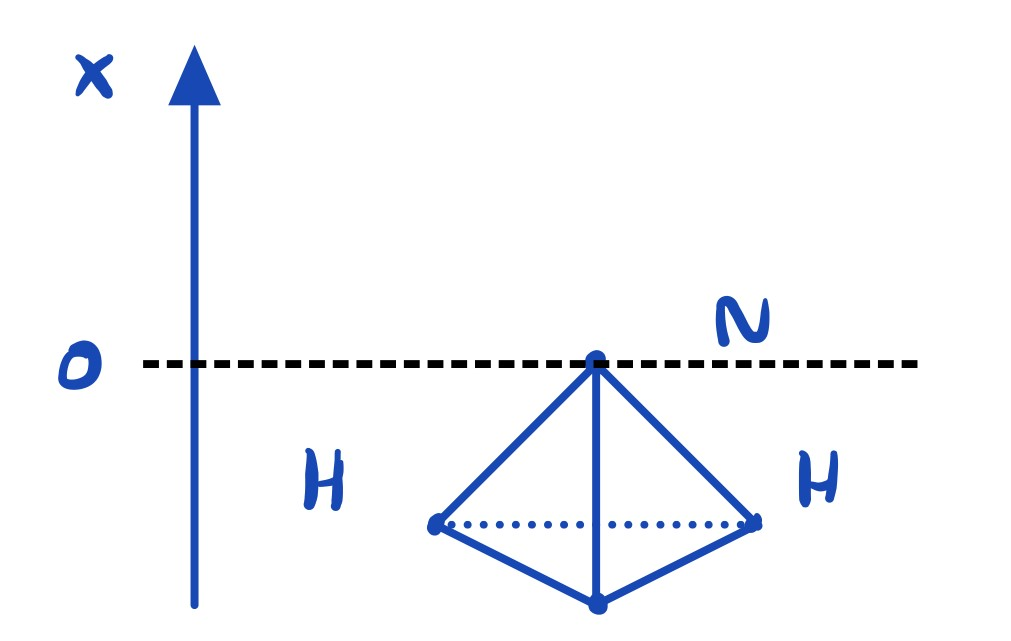
\includegraphics[width=60mm,scale=0.5]{Chapitre 5/Figure 1.jpg}
    \caption{Schéma d'une molécule d'ammoniac. La distance x désigne la distance entre le plan formé par les atomes d'hydrogène et l'atome d'azote.}
    \label{fig:Schema ammoniac}
\end{figure}

Soit $|x| = b$ la distance minimisant l'énergie potentielle. Puisque l'énergie potentielle est \emph{paire}, nous avons que $V(-b) = V(b)$. Choissons l'échelle de l'énergie de sorte que $V(b) = 0$. Nous avons alors une barrière de potentiel en $x = 0$, d'énergie $V_1 > V_0 = 0$.\\

\begin{figure}[h]
    \centering
    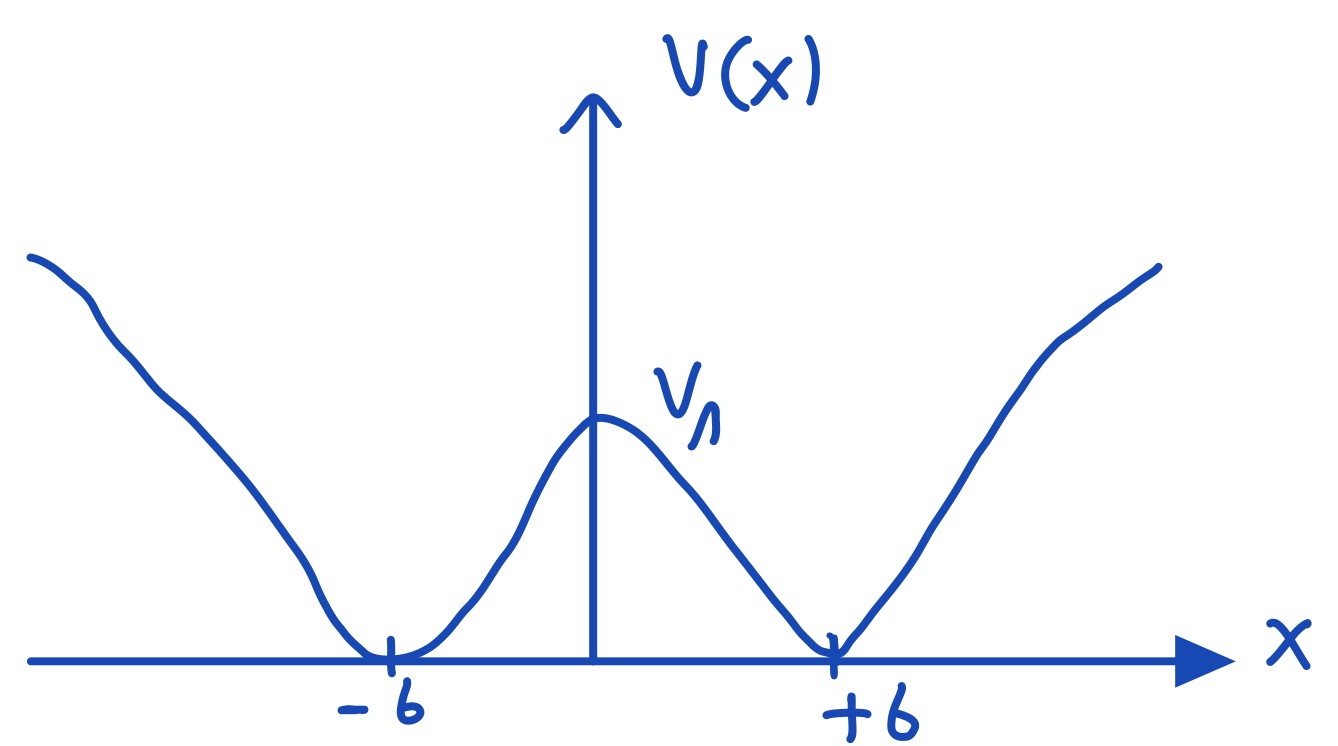
\includegraphics[width=70mm,scale=0.5]{Chapitre 5/Figure 2.jpg}
    \caption{Représentation de l'énergie potentielle en fonction de la distance $x$. On observe que lorsque $\norm{x}>b$, l'énergie augmente significativement: cela correspond à la croissance de la force de liaison chimique assurant la cohésion moléculaire. La barrière de potentiel en $x = 0$ traduit la force de répulsion entre les atomes d'hydrogène et l'atome d'azote lorsque ce dernier est dans le plan qu'ils forment.}
\end{figure}

Que prédit la mécanique quantique sur les niveaux d'énergie de ce système? Classiquement, il n'est pas possible pour une particule d'énergie inférieure à $V_1$ de franchir la barrière de potentiel placée en $x=0$. Nous aurions alors que l'atome d'azote resterai toujours du même côté du plan formé par les atomes d'hydrogène. Cependant, comme nous l'avons étudié en \ref{chap2:potentiel carre}, le phénomène d'effet tunnel autorise les états d'énergie inférieur : l'inversion de la molécule est alors une réalité quantique inexpliquée par la mécanique classique.\\

Notons par $\ket{+}$ l'état dans lequel l'atome d'azote est au-dessus des atomes d'hydrogènes, et par $\ket{-}$ lorsqu'il est en-dessous. Dans la base formé par ces deux états, l'Hamiltonien de ce système s'exprime par
\begin{equation}
    H = 
    \begin{pmatrix}
        E_0 & -A\\
        -A & E_0
    \end{pmatrix}\label{eq:Hamiltonien applications}
\end{equation}
où $E_0$ représente l'énergie fondamentale du système, et $A$ est une perturbation que l'on fait subir au système.\\

De part le postulat de la mesure, les valeurs de la mesure d'une observable sont les valeurs propres associées à celle-ci : un calcul rapide du spectre de \eqref{eq:Hamiltonien applications} permet de montrer que nous avons un
\begin{itemize}
    \item état propre $\ket{\psi_-} = \frac{1}{\sqrt{2}}\left(\ket{-}+\ket{+}\right)$ d'énergie $E_0-A$ ;
    \item état propre $\ket{\psi_+} = \frac{1}{\sqrt{2}}\left(\ket{-}-\ket{+}\right)$ d'énergie $E_0+A$.
\end{itemize}

Nous voyons alors qu'il existe une énergie, $E_0-A$, plus petite que $E_0$ : cela montre que la molécule d'ammoniac est très stable.

\subsection*{Exemple 2 : La molécule de benzène}

\color{purple} Les chimistes représentent des molécules organiques compliquées avec des schémas somme toute assez simple. Nous discutons ici d'une de ces molécules: la plus intéressante d'entre elles, la molécule de benzène. Selon les représentations utilisées par les chimistes, elle se représente par la figure suivante.

\begin{figure}[h]
    \centering
    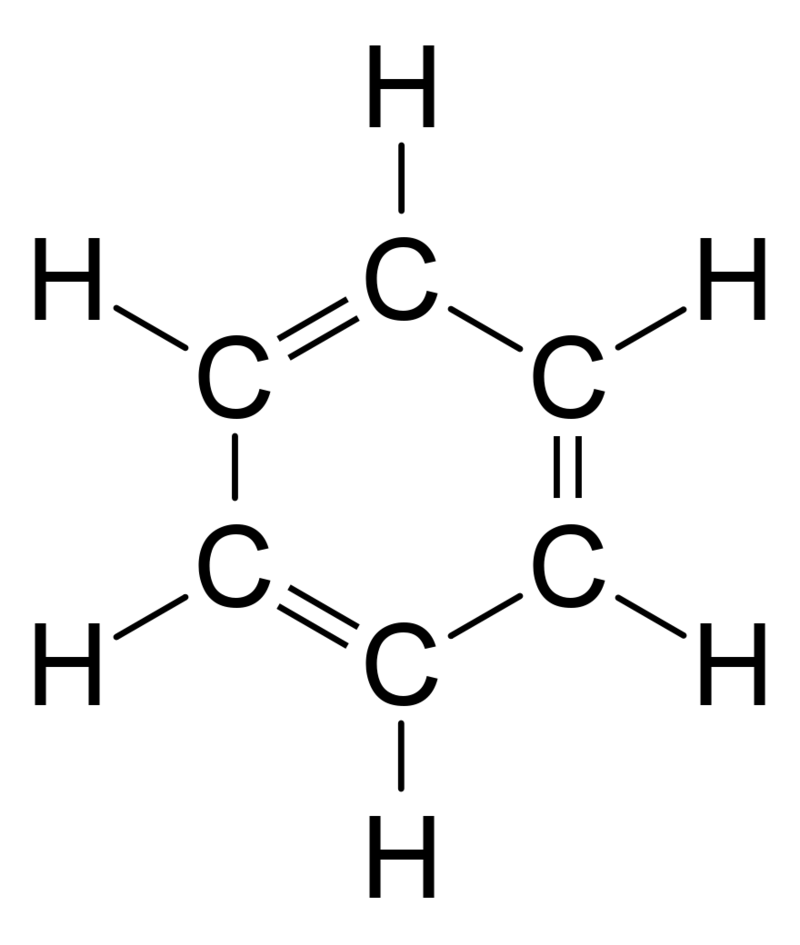
\includegraphics[width=3cm,scale=0.4]{Chapitre 5/Figure 3.png}
    \caption{Représentation d'une molécule de benzène $C_6H_6$. Une bare représente une "paire" d'électrons dans une liaison covalente - de même, les doubles bares correspondent à une double paire d'électrons impliquées dans la liaison.}
    \label{fig:molecule de benzene}
\end{figure}

Cette molécule est intéressante sur plusieurs niveaux: nous avons par exemple que l'énergie théorique nécessaire pour former la molécule (calculée en effectuant la somme de l'énergie des composants) est plus petite que l'énergie expérimentalement mesurée. Nous allons nous intéresser ici à un autre aspect de cette molécule. En regardant la figure \ref{fig:molecule de benzene}, on observe qu'il y a un totale de 3 double liaisons. Deux double liaisons à gauche, et une à doite. Rien ne nous empêche, à priori, de faire l'inverse: une double liaison à gauche, et deux double liaisons à droite. Cela donnerait quelque chose comme représenté par la figure \ref{fig:symmetrie benzene}.

\begin{figure}[h]
    \centering
    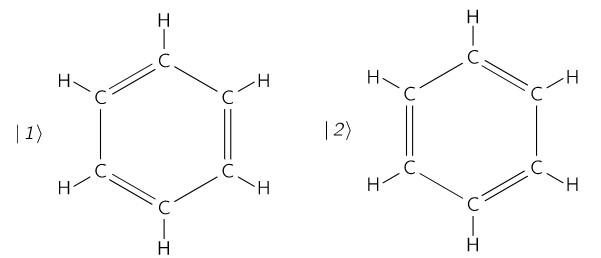
\includegraphics[width=6cm,scale=0.5]{Chapitre 5/Figure 4.jpg}
    \caption{Parallèle entre les deux types de molécule de benzène possible.}
    \label{fig:symmetrie benzene}
\end{figure}

Les deux molécules étant la même, elles devraient avoir la même énergie. Nous devons alors les analyser comme un système à deux  niveaux: chaque état représente une configuration possible de l'ensemble des électrons, et il existe une probabilité non nulle que l'ensemble passe d'une configuration à l'autre. \color{black}Notons par $\ket{1}$ la première disposition possible, et par $\ket{2}$ la seconde. Dans la base orthonormale formée par ces états, l'Hamiltonien décrivant le système est à nouveau donné par \eqref{eq:Hamiltonien applications}. L'état de plus basse énergie est alors à nouveau donnée par $\ket{\psi_-} = \frac{1}{\sqrt{2}}\left(\ket{1}+\ket{2}\right)$, d'énergie $E_0-A$. Cette énergie étant plus faible que $E_0$, nous avons à nouveau une indication de la stabilité de la molécule de benzène.

\subsection*{Exemple 3 : Ion moléculaire $H_2^+$}

Pour finir, considérons deux protons séparés par une distance $r$, ainsi qu'une particule d'électron qui peut soit être dans le voisinage du proton de gauche, soit dans le voisinage du proton de droite.\\

\begin{figure}[h]
    \centering
    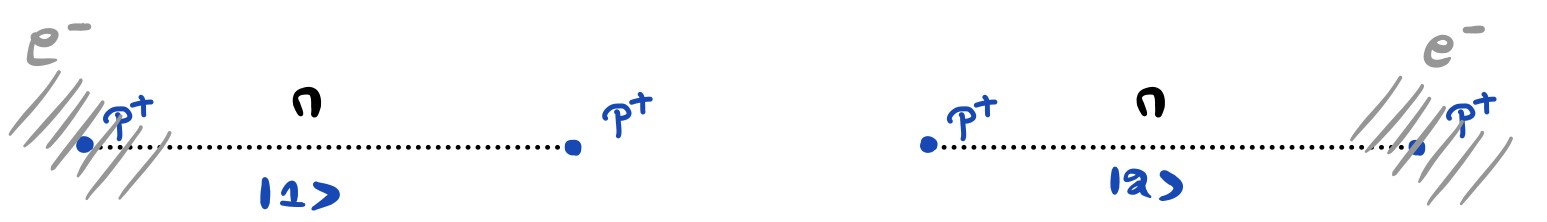
\includegraphics[width=9cm,scale=0.9]{Chapitre 5/Figure 5.jpg}
    \caption{Mise en parallèle des deux positions possible de l'électron : soit à gauche, dans l'état $\ket{1}$, soit à droite, dans l'état $\ket{2}$.}
\end{figure}

Classiquement, une fois que l'électron est stable dans une des deux situations, elle ne peut se retrouver dans l'autre : nous pouvons voir cela en analysant les forces électromagnétiques s'appliquant à l'électron. Quantiquement, l'électron peut librement se déplacer d'un voisinage à l'autre : il s'agit une fois de plus d'une application de l'\textit{effet tunnel}.\\

Nous pouvons à nouveau appliquer l'Hamiltonien \eqref{eq:Hamiltonien applications} à cette situation, à une petite modification clée: $E_0(r)$ et $A(r)$ dépendent ici de la distance $r$ entre les deux protons. Nous avons donc
\begin{equation}
    H(r) = \begin{pmatrix}
        E_0(r) & -A(r)\\
        -A(r) & E_0(r)
    \end{pmatrix}
\end{equation}

où $E_0(r)$, lorsque les atomes sont proches, décrit la répulsion entre les protons.\\

Dans ce modèle, nous avons alors que l'état fondamental est $\frac{1}{\sqrt{2}}\left(\ket{1}+\ket{2}\right)$, d'énergie $E_-(r) = E_0(r)-A(r)$, et que l'état excité est donné par $\frac{1}{\sqrt{2}}\left(\ket{1}-\ket{2}\right)$, d'énergie $E_+(r) = E_0(r)+A(r)$. \emph{Ce modèle, naïf, forme la base de la compréhension des modèles chimiques}. \color{purple} La figure \ref{fig:comparaison E+ et E-} donne une idée de l'allure de $E_-(r)$ et de $E_+(r)$.\color{black}

\begin{figure}[h]
    \centering
    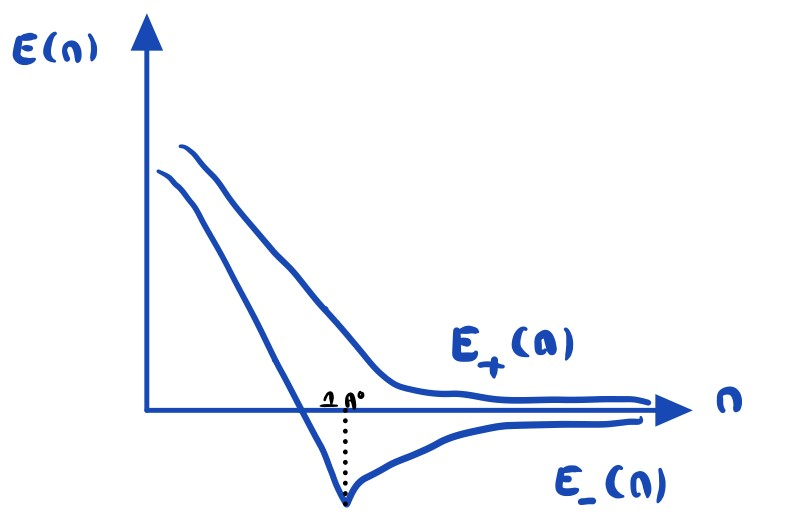
\includegraphics[width=7cm,scale=0.5]{Chapitre 5/Figure 6.jpg}
    \caption{Représentation et mise en parallèle de l'évolution de $E_-(r)$ et $E_+(r)$.}
    \label{fig:comparaison E+ et E-}
\end{figure}

\section{Spin $\frac{1}{2}$}
Ce chapitre consistue une brève introduction à la quantification du moment angulaire. Débutons par une introduction au concept de groupes de rotations.

\subsection{Groupe de rotations}

Considérons l'ensemble des matrices $R \in \mathbb{R}^{3\times 3}$ telle que $R^TR = \mathbb{I}$. Si $\bm{n}$ est un vecteur unitaire de $\mathbb{R}^3$ et $\theta$ un angle, alors $R(\theta,\bm{n}$) est la rotation (dans le sens trigonométrique) autour de l'axe $\bm{n}$ d'angle $\theta$.

\begin{align*}
    R(\theta,x) &= \begin{pmatrix}
    1 & 0 & 0\\
    0 & \cos\theta & -\sin\theta\\
    0 & \sin\theta & \cos\theta
    \end{pmatrix} = \exp (i\theta L_x)			&\text{où } L_x &= \begin{pmatrix}
    0 & 0 & 0\\
    0 & 0 & i\\
    0 & -i & 0
    \end{pmatrix}\\
    R(\theta,y) &= \begin{pmatrix}
    \cos\theta & 0 & \sin\theta\\
    0 & 1 & 0\\
    -\sin\theta & 0 & \cos\theta\\
    \end{pmatrix} = \exp(i\theta L_y)		&\text{où } L_y &= \begin{pmatrix}
    0 & 0 & -i\\
    0 & 0 & 0\\
    i & 0 & 0
    \end{pmatrix}\\
    R(\theta,z) &= \begin{pmatrix}
    \cos\theta & -\sin\theta & 0\\
    \sin\theta & \cos\theta & 0\\
    0 & 0 & 1
    \end{pmatrix} = \exp(i\theta L_z)		&\text{où } L_z &= \begin{pmatrix}
    0 & i & 0\\
    -i & 0 & 0\\
    0 & 0 & 0
    \end{pmatrix}
\end{align*}
Nous avons alors que $R(\theta,\bm{n}) = \exp (i\theta\bm{n}\cdot\bm{L})$, où $\bm{n}\cdot\bm{L} = n_iL_i$. Les vecteurs $L_x,L_y,L_z$ sont les \emph{générateurs du $\mathcal{G}$roupe des $\mathcal{R}$otations}.

\begin{Property}
    Les générateurs du groupe des rotations commutent selon
    \begin{equation}
        [L_i,L_j] = L_k
    \end{equation}
    pour tout $i,j \neq k$. 
\end{Property}

En physique, de nombreux objets (et non pas seulement les vecteurs) sont invariants ou se transforment sous l'effet d'une rotation. Une autre représentation du $\mathcal{G}$roupe des $\mathcal{R}$otations est l'ensemble des 3 opérateurs $J_x,J_y,J_z$ tels que $[J_x,J_y] = J_z$ (et toutes ses permutations cycliques) et tel que, sous toute rotation d'angle $\theta$ autour de $\bm{n}$, un état $\ket{\psi}$ se transforme en
\begin{equation}
\ket{\psi} \rightarrow \exp(i\theta\bm{n}\cdot\bm{J})\ket{\psi}
\end{equation}

\begin{exemple}Les opérateurs
\begin{itemize}
\item $J_x = yp_z - zp_y$
\item $J_y = zp_x - xp_z$
\item $J_z = xp_y - yp_x$
\end{itemize}
sont des exemples de représentation du $\mathcal{G}$roupe des $\mathcal{R}$otations.
\end{exemple}
Un système est invariant par rotation si
\begin{align}
\exp (-itH) \exp (i\theta \bm{n}\cdot\bm{J})\ket{\psi} &= \exp (i\theta \bm{n}\cdot\bm{J})\exp (-itH) \ket{\psi}			&\forall \ket{\psi},\forall \bm{n},\theta,t
\end{align}
Cela revient à dire que \emph{faire une rotation} et ensuite \emph{évoluer dans le temps} est identique à \emph{évoluer dans le temps} et puis \emph{faire une rotation}.

\begin{Property} 
    Pour tout petit angle sur des temps négigeables,  
    \begin{equation}
        [H,J_x] = [H,J_y] = [H,J_z] = 0.
    \end{equation}
\end{Property}
Les conséquences en sont nombreuses. Voici quelques exemples.
\begin{Property}
    Si $\ket{\psi(t)}$ est une solution de l'équation de Schrödinger \eqref{Schrodinger}, alors 
    \begin{equation}
        \frac{d}{dt}\braket{\psi(t)|J_i|\psi(t)} = 0
    \end{equation}
    Nous avons en particulier que $\braket{\psi(t)|J_i|\psi(t)} = \braket{\psi(0)|J_i|\psi(0)}$.
\end{Property}

\begin{Property}
    Si $\ket{\psi_0}$ est un vecteur propre de $J_i$ tel que $J_i\ket{\psi_0} = j\ket{\psi_0}$, alors le vecteur $\ket{\psi(t)} = e^{-iHt}\ket{\psi_0}$ est également un vecteur propre de $J_i$:
    \begin{equation}
        J_i\ket{\psi(t)} = j\ket{\psi(t)}.
    \end{equation}
\end{Property}
Le théorème d'Emmy Nöther permet de montrer que la symmétrie de rotation implique la conservation d'une quantité : le moment angulaire.


\subsection{Quantification du moment angulaire}
\begin{theorem}
Soit $[J_x,J_y] = iJ_z$. Nous avons alors que les valeurs propres de $J_z$ est un demi-entier: $0,\frac{1}{2}, 1, \frac{3}{2}, ...$.
\begin{equation*}
J_z \ket{\psi} = m\ket{\psi}
\end{equation*}
\end{theorem}

\begin{theorem}
Il existe une représentation non triviale du $\mathcal{G}$roupe des $\mathcal{R}$otations par des matrices $d\times d$. Dans ce cas, $J_z = -\frac{d}{2}, -\frac{d}{2}+1,...,+\frac{d}{2}$.
\end{theorem}
\begin{exemple}
Le cas le plus simple est celle des matrices de Pauli (matrices $2\times 2$):
\begin{center}
\begin{tabular}{c|c|c}
$\sigma_x = \begin{pmatrix}
0 & 1\\
1 & 0
\end{pmatrix}$ & $\sigma_x = \begin{pmatrix}
0 & -i\\
i & 0
\end{pmatrix}$ & $\sigma_x = \begin{pmatrix}
1 & 0\\
0 & -1
\end{pmatrix}$\\
$J_x = \frac{1}{2}\sigma_x$ & $J_y = \frac{1}{2}\sigma_y$ & $J_z = \frac{1}{2}\sigma_z$
\end{tabular}
\end{center}
Nous pouvons vérifier que les différentes relations démontrées ci-dessus sont respectées (exercice).
\end{exemple}

En particulier, nous pouvons vérifier que 
\begin{center}
    \begin{tabular}{c|c|c|c}
        $\{\sigma_a,\sigma_b\} = 2i\varepsilon_{abc}\sigma_c$ & $\{\sigma_a,\sigma_b\} = 2\sigma_{ab}\hat{I}$ & $Tr(\sigma_a) = 0$ & $\sigma_a\sigma_b = \delta_{ab}\hat{I}+i\varepsilon_{abc}\sigma_c$
    \end{tabular}
\end{center}

Les matrices de Pauli sont de valeur propres $\pm 1$. Les vecteurs propres associés sont
\begin{center}
    \begin{tabular}{c|c}
        $\psi_x^+ = \frac{1}{\sqrt{2}} \begin{pmatrix}
            1\\
            1
        \end{pmatrix}$ & $\psi_x^- = \frac{1}{\sqrt{2}} \begin{pmatrix}
            -1\\
            1
        \end{pmatrix}$\\
        $\psi_y^+ = \frac{1}{\sqrt{2}} \begin{pmatrix}
            -1\\
            1
        \end{pmatrix}$ & $\psi_y^- = \begin{pmatrix}
            i\\
            i
        \end{pmatrix}$\\
        $\psi_z^+ = \begin{pmatrix}
            1\\
            0
        \end{pmatrix} = \ket{\uparrow}$ & $\psi_z^- = \begin{pmatrix}
            0\\
            1
        \end{pmatrix} = \ket{\downarrow}$
    \end{tabular}
\end{center}

Introduisons le vecteur unitaire associé aux coordonnées sphériques $\bm{n} = \left(\sin\theta\cos\varphi,\sin\theta\sin\varphi,\cos\theta\right)$. Observons que 
\begin{equation}
    \bm{n}\cdot\bm{\sigma} = \begin{pmatrix}
        \cos\theta & \sin\theta e^{-i\varphi}\\
        \sin\theta e^{i\varphi} & -\cos\theta
    \end{pmatrix}
\end{equation}
De même, observons que $\begin{pmatrix}
    \cos\frac{\theta}{2}\\
    \sigma\frac{\theta}{2}e^{i\varphi}
\end{pmatrix}$ est le vecteur propre de valeur propre $+1$. Nous pouvons réécrire, dans la base des vecteurs up and down,
\begin{equation}
    \begin{pmatrix}
        \cos\frac{\theta}{2}\\
        \sigma\frac{\theta}{2}e^{i\varphi}
    \end{pmatrix} = \cos\frac{\theta}{2}\ket{\uparrow}+\sin\frac{\theta}{2}e^{i\varphi}\ket{\downarrow}
\end{equation}

Les particules élémentaires ont un spin $1/2$. Elles sont munies d'un espace de Hilbert de dimension 2, se transformant sous rotations par $e^{i\frac{\theta}{2}\bm{n}\cdot\bm{\sigma}}$.

\end{document}